\documentclass[11pt]{article}
\usepackage[review]{acl}
\usepackage{times}
\usepackage{latexsym}
\usepackage{amsmath}
\usepackage{amssymb}
\usepackage{amsthm}
\usepackage{booktabs}
\usepackage{multirow}
\usepackage{graphicx}
\usepackage{subcaption}
\usepackage{algorithm}
\usepackage{algpseudocode}
\usepackage{microtype}
\usepackage{cleveref}

\setlength{\textfloatsep}{7pt plus 2pt minus 2pt}
\setlength{\floatsep}{6pt plus 2pt minus 2pt}
\setlength{\intextsep}{6pt plus 2pt minus 2pt}
\setlength{\dbltextfloatsep}{8pt plus 2pt minus 2pt}
\setlength{\dblfloatsep}{6pt plus 2pt minus 2pt}

\newtheorem{theorem}{Theorem}
\newtheorem{lemma}[theorem]{Lemma}
\newtheorem{definition}{Definition}

\title{\textbf{SPADE: Evidence-Selective Draft Context Speculative Decoding\\for Knowledge-Intensive Generation}}

\author{Anonymous ACL submission}

\date{}

\begin{document}
\maketitle

\begin{abstract}
Speculative decoding accelerates LLM inference via parallel verification, yet over long retrieved contexts ($5\text{k}$--$18\text{k}$ tokens) full drafting inflates draft KV-cache memory ($M_{\text{KV}} \propto S$) and prefill compute ($O(S^2)$), while naive passage pruning drops critical facts and stalls acceptance. We present \textbf{SPADE}, a distribution-preserving asymmetric speculative decoding framework: the target verifier retains full context to preserve the target distribution via residual verification (Theorem \ref{thm:invariance}), while the draft model conditions on a compact sentence-budgeted context selected via upper-layer target attention weights captured during target prefill with no auxiliary forward pass ($0.163\text{ ms/tok}$ amortized). On 300 held-out AVeriTeC claims (\texttt{Qwen3-8B/0.6B}, RTX 5090), SPADE reaches \textbf{43.28 tok/s} (\textbf{+22.4\%} vs.\ AR, \textbf{+4.4\%} vs.\ Full-SD, $p_{\text{Holm}} < 10^{-4}$), cuts active draft KV by \textbf{$-63.9\%$}, and preserves acceptance ($78.20\%$ vs.\ $78.16\%$). On all $173$ long claims ($>10\text{k}$ chars), SPADE outperforms SnapKV-style \texttt{KV-Sparse} ($+2.09\text{ tok/s}$, $p_{\text{Holm}} < 10^{-4}$) and Prompt-Lookup ($+10.54\text{ tok/s}$), matches zero-GPU BM25 sentence budgeting in wall-clock speed, and improves acceptance ($+0.96\text{ pp}$ overall, $p_{\text{Holm}}=0.0066$). SPADE transfers to \texttt{Qwen2.5-7B/0.5B} ($+11.7\%$ vs.\ AR, $-63.8\%$ KV) and \textbf{LongBench HotpotQA} ($N=100$, mean $14,083$ tok: $-79.7\%$ draft KV, $+1.37\text{ tok/s}$ vs.\ Full-SD, $p_{\text{Holm}} < 10^{-4}$, preserved QA F1/Sub-EM), while $16\text{k}$--$32\text{k}$ scaling analysis identifies when target KV traffic dominates beyond $\sim 14\text{k}$ tokens.
\end{abstract}

\section{Introduction}
\label{sec:intro}

Autoregressive inference in modern Transformer large language models (LLMs) is fundamentally constrained by high-bandwidth memory (HBM) latency: generating each token requires streaming multi-billion parameter matrices through compute cores for a single vector-matrix multiply \citep{shazeer2019fast,leviathan2023fast,chen2023accelerating}. Speculative decoding amortizes this memory bandwidth bottleneck by employing a lightweight draft model to autoregressively propose $K$ candidate tokens, which are verified simultaneously by the target model in a single parallel forward execution.

In knowledge-intensive generation tasks---such as multi-document question answering and real-world claim verification \citep{schlichtkrull2023averitec,thorne2018fever}---prompts are dominated by extensive retrieved evidence documents ($5\text{k}$--$8\text{k}+$ tokens). Under this long-context regime, standard speculative decoding encounters two critical dilemmas:
\begin{enumerate}
    \item \textbf{Draft KV Cache Memory Bloat:} Feeding full retrieved passages into the draft model inflates active key-value (KV) cache memory footprints linearly ($M_{\text{KV}} \propto S$), while prompt prefill compute scales quadratically ($O(S^2)$). During decode phase, streaming larger KV caches linearly increases per-step memory traffic ($O(S)$), eroding net speculative acceleration.
    \item \textbf{Failure Modes of Document Pruning:} Naive document pruning (e.g., retaining top-$k$ BM25 passages for the drafter) degrades proposal quality: when critical evidence resides in dropped passages, the draft model generates mismatched tokens that the target model rejects, degrading proposal acceptance by up to $-5.7\text{ pp}$ and stalling generation throughput.
\end{enumerate}

\begin{figure*}[t]
\centering
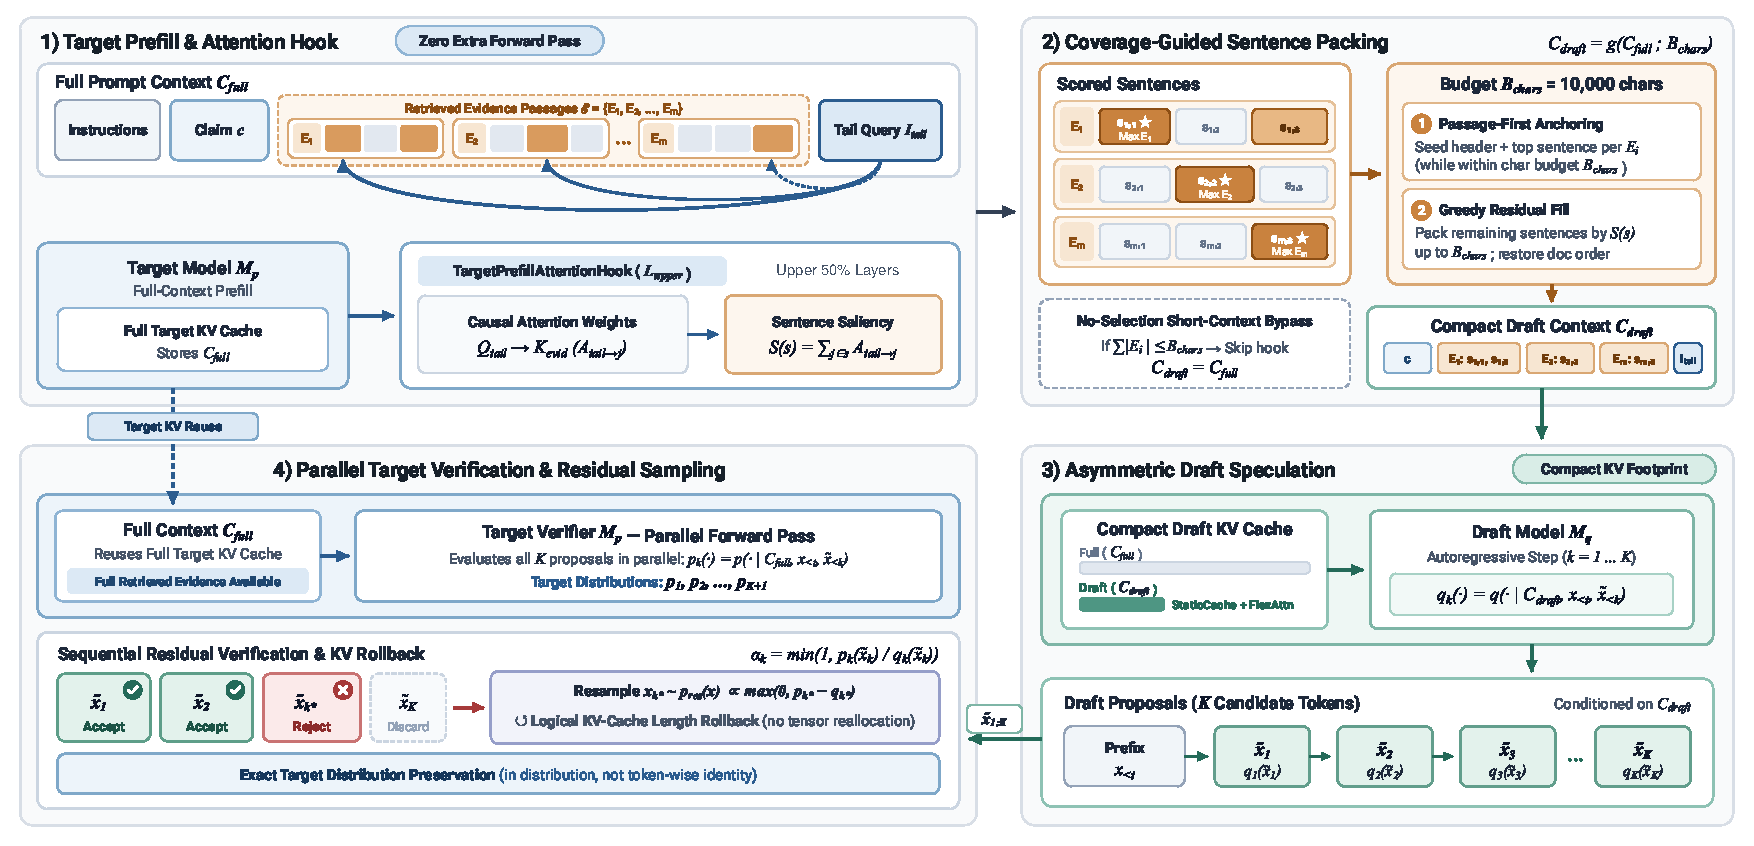
\includegraphics[width=0.90\textwidth]{figures/spade_overview.pdf}
\caption{\textbf{SPADE Overview:} (1) Target prefills $C_{\text{full}}$; (2) \texttt{TargetPrefillAttentionHook} scores sentences from upper-layer terminal queries ($0.163\text{ ms/tok}$ amortized, zero extra forward passes); (3) Greedy packing under budget $B$ with per-passage coverage ($m/m$) trims $\sim$65\% draft tokens (bypassing short inputs); (4) Compiled FlexAttention/StaticCache drafter proposes $K$ tokens verified via residual sampling (Theorem \ref{thm:invariance}).}
\label{fig:spade_overview}
\end{figure*}

To overcome this, we present \textbf{SPADE} (\textbf{S}peculative \textbf{P}rompt \textbf{A}ttention-\textbf{D}rafted \textbf{E}vidence), an \textbf{asymmetric evidence context architecture} decoupling target verification from draft proposal. The target retains $C_{\text{full}}$ to preserve its distribution under residual verification (Theorem \ref{thm:invariance}), while the drafter conditions on sentence-budgeted evidence $C_{\text{draft}} = g(C_{\text{full}}; B)$ ($B = 10\text{k}$) scored via a lightweight target-prefill hook ($0.163\text{ ms/tok}$) under a per-passage coverage constraint ($m/m$).

The primary contributions of this paper are:
\begin{itemize}
    \item \textbf{Target-Prefill Attention-Guided Sentence Selection:} A lightweight hook ($0.163\text{ ms/tok}$) extracting upper-layer causal attention during target prefill, paired with greedy packing and a per-passage coverage constraint ($m/m$) with no auxiliary passes.
    \item \textbf{Asymmetric Speculative Formulation:} Conditioning the drafter on $C_{\text{draft}} = g(C_{\text{full}}; B)$ while verifying against $C_{\text{full}}$ preserves the target distribution (Theorem \ref{thm:invariance}), verified via seed-noise and teacher-forced audits.
    \item \textbf{Controlled Empirical Acceleration:} On 300 AVeriTeC claims, SPADE reaches \textbf{43.28 tok/s} ($+22.4\%$ vs.\ AR, $+4.4\%$ vs.\ Full-SD, $p_{\text{Holm}} < 10^{-4}$), cuts draft KV \textbf{$-63.9\%$}, preserves acceptance ($78.20\%$ vs.\ $78.16\%$), and beats \texttt{KV-Sparse} ($+2.09\text{ tok/s}$) and \texttt{PLD} ($+10.54\text{ tok/s}$) on $N=173$ long claims.
    \item \textbf{Cross-Model \& Cross-Task Generalization:} SPADE transfers to \texttt{Qwen2.5-7B/0.5B} ($+11.7\%$ vs.\ AR, $-63.8\%$ KV) and \textbf{LongBench HotpotQA} ($N=100$, mean $14,083$ tok: $-79.7\%$ KV, $+1.37\text{ tok/s}$ vs.\ Full-SD, $p_{\text{Holm}} < 10^{-4}$; preserved QA F1/Sub-EM) while identifying target-KV dominance beyond $14\text{k}$--$16\text{k}$ tokens.
\end{itemize}

\section{Related Work}
\label{sec:related}

\paragraph{Speculative Decoding with Sparse or Asymmetric Contexts:}
Speculative execution for autoregressive LLMs was formalized by \citet{leviathan2023fast} and \citet{chen2023accelerating}, proving that an auxiliary draft model $q$ can propose candidate tokens verified in parallel by a target model $p$ without altering the target distribution. While classical speculative formulations assume identical prompts for draft and target models, several recent systems incorporate asymmetric context representations: TriForce \citep{sun2024triforce} and MagicDec \citep{chen2024magicdec} accelerate drafting via hierarchical or sparse KV caches where the drafter attends over streaming/pruned KV states while the verifier accesses full context. Other approaches explore dynamic draft horizons \citep{zhang2025draftstop,wang2026linguaspec}, training-free prompt-lookup matching \citep{saxena2023promptlookup}, or KV token eviction \citep{li2024snapkv}. In contrast to internal KV-cache eviction or trained constant-KV draft architectures, SPADE operates cleanly at the \textit{textual sentence level} for unmodified off-the-shelf draft models, extracting target-prefill attention weights to construct an evidence-budgeted prompt with a per-passage coverage constraint ($m/m$).

\paragraph{Context Compression vs.\ Distribution Preservation:}
Prompt compression methods such as LLMLingua \citep{jiang2023llmlingua} and RECOMP \citep{xu2023recomp} shorten input text directly for the primary model, modifying target hidden states and risking task accuracy degradation. In contrast, SPADE compresses evidence context \textit{only for the draft model}; the target model retains the full uncompressed context, preserving target distribution invariance under the residual verification criterion.

\paragraph{Long-Context Asymmetric Drafting:}
Recent methods explore distinct points in the long-context design space. RAPID \citep{chen2025rapid} pairs a dense-retrieval RAG drafter (enabling same-scale speculation) with inference-time logit enrichment that modifies the target distribution. SpecExtend \citep{cha2025specextend} combines FlashAttention/hybrid tree attention with cross-model KV retrieval dynamically updating draft KV states from target attention scores. LongSpec \citep{yang2025longspec} introduces a trained constant-KV draft architecture with specialized position indices for short-to-long adaptation and hybrid tree attention. Conversely, AsymSpec \citep{liang2026asymspec} applies the reverse asymmetry to agentic pipelines---running a lightweight full-context drafter against a compressed verifier via contrastive logit fusion ($\approx 90\%$ full-context accuracy). Distinct from these trained or KV-evicting mechanisms, SPADE targets multi-document knowledge-intensive generation with unmodified drafters, training-free target-prefill sentence selection, and an empirical evaluation against KV-sparse and prompt-lookup baselines.

\section{Empirical Diagnosis: Why Passage-Level Context Reduction Fails}
\label{sec:diagnosis}

To investigate why conventional context reduction fails in speculative decoding, we profiled 100 long-context claim verification prompts from the exploratory development set (\texttt{train-retrieved-bounded}, mean prompt length 6,153 tokens; distinct from our frozen held-out test split in Section \ref{sec:experiments}).

\paragraph{Failure Modes of Document Pruning:}
A natural baseline is coarse document pruning: providing the drafter only the top-2 retrieved passages via BM25 (\texttt{BM25 Top-2}). While this sheds 40.8\% of prompt text, empirical acceptance drops by $-1.8\text{ pp}$ overall and by $-5.7\text{ pp}$ on dense claims ($m \ge 3$ passages). In multi-document fact-checking, claims frequently require synthesizing evidence scattered across multiple sources. When the drafter lacks a dropped passage, its draft proposals diverge from the target distribution, triggering early target verification rejections and eroding speculative throughput.

\paragraph{The Sentence-Level Compression Opportunity:}
Micro-profiling revealed that within retrieved passages, target model attention is highly concentrated: claim query tokens attend strongly to only $31.8\%$ of evidence sentences, while the remaining $68.2\%$ exhibit low attention mass. This establishes the central insight of SPADE: by selecting salient sentences across \textit{all} passages rather than dropping entire passages, we can compress draft prompt length by $>60\%$ while preserving 100\% passage coverage and critical reasoning cues.

\section{The SPADE Framework}
\label{sec:method}

\subsection{Asymmetric Speculative Formulation}
Let $x_{<t}$ denote the sequence generated up to step $t$. Let $C_{\text{full}}$ denote the complete prompt containing all retrieved evidence passages $\mathcal{E} = \{E_1, \dots, E_m\}$, and let $C_{\text{draft}} = g(C_{\text{full}}; B)$ denote the compact draft context constructed under budget $B$, where $g$ denotes the evidence selection and repackaging function.
At speculative round $j$, the draft model proposals $\tilde{x}_1, \dots, \tilde{x}_K$ are generated autoregressively conditioned on $C_{\text{draft}}$:
\begin{equation}
q_k(\cdot) = q(\cdot \mid C_{\text{draft}}, x_{<t}, \tilde{x}_{<k}), \quad k \in \{1, \dots, K\}
\end{equation}
The target model verifies all $K$ candidates in a single parallel forward pass conditioned on $C_{\text{full}}$:
\begin{equation}
p_k(\cdot) = p(\cdot \mid C_{\text{full}}, x_{<t}, \tilde{x}_{<k}), \quad k \in \{1, \dots, K+1\}
\end{equation}

\subsection{Target-Prefill Attention Hook}
To identify salient evidence sentences without auxiliary neural models or extra forward passes, SPADE captures causal self-attention during the target model's initial prompt prefill pass.

In autoregressive decoder-only LLMs, prompt tokens are causally masked: tokens cannot attend to subsequent positions. The input prompt is structured as $\text{Instructions} \to \text{Claim } c \to \text{Evidence } \mathcal{E} \to \text{Trigger } \tau$ (e.g., \texttt{JSON: \{"summary":"...}). To ensure query tokens have full causal visibility over all evidence passages $\mathcal{E}$, SPADE hooks the \textit{terminal query window} $I_{\text{tail}} = \{P - W + 1, \dots, P\}$ ($W=16$ tokens, prompt length $P$). Because $I_{\text{tail}}$ follows all evidence passages, its queries $Q_{\text{tail}}$ causally attend to all preceding evidence keys $K_{\text{evidence}}$.

Crucially, modern inference engines use fused attention kernels (e.g., FlashAttention or PyTorch SDPA) that do not materialize the $P \times P$ attention matrix. Instead of requiring an unfused full forward pass, SPADE registers a lightweight pre-hook on the self-attention modules of upper layers $L_{\text{upper}}$ (upper 50\% of layers, $\{L/2, \dots, L-1\}$), capturing only the final $W=16$ hidden states $h_{\text{tail}}$ and RoPE cosine/sine embeddings. After target prefill populates the standard key-value cache, SPADE projects $h_{\text{tail}}$ via $W_q$, applies per-head QK-Norm (when present, e.g., \texttt{Qwen3}) and RoPE, broadcasts across grouped-query attention (GQA) key heads, applies the bottom-right $W \times W$ causal mask, and computes FP32 softmax over $W \times P$ scores against cached keys $K \in \mathbb{R}^{P \times d}$:
\begin{equation}
A_{\text{tail} \to j} = \frac{1}{|L_{\text{upper}}|} \sum_{l \in L_{\text{upper}}} \frac{1}{H} \sum_{h=1}^H \frac{1}{W} \sum_{i \in I_{\text{tail}}} \left[\text{Softmax}\left(\frac{Q_{l, i}^h K_{l}^{h\top}}{\sqrt{d_k}}\right)\right]_j
\end{equation}
Because $W=16 \ll P$, hook computation scales linearly as $O(W \cdot P)$ rather than $O(P^2)$: across $P \in [2\text{k}, 32\text{k}]$ on \texttt{Qwen3-8B} (18 hooked layers), measured peak allocator delta VRAM scales from $19.1\text{ MB}$ ($6.5\text{ ms}$) at $2\text{k}$ to $73.7\text{ MB}$ ($9.2\text{ ms}$) at $8\text{k}$ and $291.0\text{ MB}$ ($30.6\text{ ms}$) at $32\text{k}$ tokens---roughly an order of magnitude smaller than unfused $P \times P$ matrices---while amortizing to $0.163\text{ ms/tok}$ on our 300-claim workload. Direct verification against eager \texttt{output\_attentions=True} confirms numerical faithfulness: worst-case max error is $5.96 \times 10^{-8}$ on \texttt{Qwen3-0.6B} (FP32, Pearson $r = 1.0000$), and mean $r = 0.99999$ ($\min$ Spearman $\rho = 0.9998$, $99.1\%$ top-64 token overlap) on \texttt{Qwen3-8B} BF16 (Appendix \ref{app:hardware}). For each candidate sentence $s \in \mathcal{E}$ spanning token indices $[s_{\text{start}}, s_{\text{end}})$, its saliency score $S(s)$ is the aggregated attention mass across its tokens:
\begin{equation}
S(s) = \sum_{j = s_{\text{start}}}^{s_{\text{end}} - 1} A_{\text{tail} \to j}
\end{equation}

\subsection{Sentence-Level Greedy Packing}
Given sentence scores $\{S(s)\}$ and a character budget $B$ ($10\text{k}$ characters):
\begin{enumerate}
    \item \textbf{Per-Passage Coverage Constraint ($m/m$):} For each passage $E_i \in \mathcal{E}$, we select the sentence with the highest saliency score $\arg\max_{s \in E_i} S(s)$ and preserve its original passage header.
    \item \textbf{Greedy Residual Packing:} Remaining sentences across all passages are ranked globally by $S(s)$ and greedily packed until reaching budget $B$.
    \item \textbf{Minimal-Overhead Bypass:} If total evidence length $\sum_{i} |E_i| \le B$, SPADE bypasses selection and sets $C_{\text{draft}} = C_{\text{full}}$ with negligible overhead ($2.45\,\mu\text{s}$ per claim).
\end{enumerate}

\subsection{Exact Speculative Sampling}
Each candidate $\tilde{x}_k$ is evaluated sequentially via the exact speculative criterion \citep{leviathan2023fast}:
\begin{equation}
\alpha_k = \min\left(1, \frac{p_k(\tilde{x}_k)}{q_k(\tilde{x}_k)}\right)
\end{equation}
Candidate $\tilde{x}_k$ is accepted if $r_k \sim \mathcal{U}[0, 1] \le \alpha_k$. If candidate $k^*$ is rejected, speculation terminates and a replacement token is sampled from the residual distribution:
\begin{equation}
p_{\text{res}}(x) = \frac{\max(0, p_{k^*}(x) - q_{k^*}(x))}{\sum_{x'} \max(0, p_{k^*}(x') - q_{k^*}(x'))}
\end{equation}

\begin{theorem}[Target Distribution Invariance]
\label{thm:invariance}
Following the exact speculative residual sampling formulation of \citet{leviathan2023fast}, for any draft prompt $C_{\text{draft}}$ and target prompt $C_{\text{full}}$, sampling tokens under the residual criterion produces token sequences distributed identically to autoregressive sampling from $p(\cdot \mid C_{\text{full}})$ under temperature $T$ and nucleus (top-$p$) filtering. This establishes mathematical distribution equivalence over candidate token probabilities, distinct from bitwise deterministic RNG matching across differing hardware execution graphs.
\end{theorem}
\begin{proof}
Let $p(x)$ and $q(x)$ abbreviate $p_k(x)$ and $q_k(x)$. The marginal probability of emitting token $x$ is:
$P(X=x) = q(x) \min(1, \frac{p(x)}{q(x)}) + \left(1 - \sum_{x'} \min(q(x'), p(x'))\right) \frac{\max(0, p(x)-q(x))}{\sum_{x'} \max(0, p(x')-q(x'))} = \min(q(x), p(x)) + \max(0, p(x)-q(x)) = p(x)$. Thus, the target distribution is strictly preserved.
\end{proof}

\begin{algorithm}[t]
\caption{SPADE Speculative Decoding}
\label{alg:spade}
\small
\begin{algorithmic}[1]
\Require Target $M_p$, Draft $M_q$, Evidence $\mathcal{E}$, Claim $c$, Budget $B$, Horizon $K$.
\State $C_{\text{full}} \gets \text{FormatPrompt}(c, \mathcal{E})$
\If{$\sum_i |E_i| \le B$}
    \State $C_{\text{draft}} \gets C_{\text{full}}$ \Comment{Minimal-overhead bypass}
    \State Prefill $M_p(C_{\text{full}})$ and $M_q(C_{\text{draft}})$
\Else
    \State Attach \texttt{TargetPrefillAttentionHook} to $M_p$
    \State Prefill $M_p(C_{\text{full}})$; extract scores $\{S(s)\}$
    \State $C_{\text{draft}} \gets \text{GreedyPack}(\mathcal{E}, \{S(s)\}, B)$
    \State Prefill $M_q(C_{\text{draft}})$
\EndIf
\While{not generated $[EOS]$}
    \State Sample $K$ draft tokens $\tilde{x}_{1:K} \sim M_q(\cdot \mid C_{\text{draft}})$
    \State Evaluate $p_{1:K+1}$ in parallel via $M_p(\cdot \mid C_{\text{full}})$
    \State Apply exact residual verification (Eq. 5--6)
    \State Rollback rejected KV cache slots in $M_q$ and $M_p$
\EndWhile
\end{algorithmic}
\end{algorithm}

\begin{table*}[t]
\centering
\small
\resizebox{\textwidth}{!}{%
\begin{tabular}{llccccccccc}
\toprule
\textbf{Decoding Method} & \textbf{Context Policy} & \textbf{Mean Draft Tok} & \textbf{Active Draft KV} & \textbf{Peak GPU VRAM} & \textbf{$\alpha_{\text{eval}}$ (\%)} & \textbf{Tok/Rnd} & \textbf{Decode Thpt} & \textbf{E2E Thpt} & \textbf{E2E Latency} & \textbf{$\Delta$ vs. Full (95\% CI)} \\
\midrule
\textbf{B0-S (Target AR)} & Full (Target Only) & — & — & 19.48 GB & — & 1.000 & 43.08 & 35.35 & 28.29 & -6.12 [-7.78, -4.70]$^*$ \\
\textbf{Baseline Full} & Full $\to$ Full & 5,090.1 & 566.9 MB & 22.57 GB & 78.16\% & 3.106 & 55.39 & 41.47 & 24.12 & — \\
\textbf{BM25 Top-2} & Full $\to$ Top-2 & 2,228.4 & 253.9 MB & 21.15 GB & 76.67\% & 3.014 & 54.64 & 41.89 & 23.87 & +0.42 [-0.08, +0.89] \\
\textbf{BM25 Sent-B8k} & Full $\to$ Sent B=8k & 1,383.3 & 161.5 MB & 20.92 GB & 77.36\% & 3.058 & 55.91 & 42.69 & 23.42 & +1.22 [+0.77, +1.68]$^*$ \\
\textbf{BM25 Sent-B10k} & Full $\to$ Sent B=10k & 1,646.4 & 190.3 MB & 20.97 GB & 77.24\% & 3.047 & 55.73 & 42.65 & 23.45 & +1.19 [+0.69, +1.68]$^*$ \\
\textbf{SPADE (Ours)} & Full $\to$ Attn B=10k & \textbf{1,776.8} & \textbf{204.6 MB} & \textbf{21.23 GB} & \textbf{78.20\%} & \textbf{3.114} & \textbf{57.03} & \textbf{43.28} & \textbf{23.10} & \textbf{+1.82 [+1.39, +2.23]$^*$} \\
\bottomrule
\end{tabular}%
}
\caption{\textbf{Main Decoding Efficiency \& Memory Matrix ($N=300$ AVeriTeC Claims, RTX 5090):} Throughput in tok/s; latency in ms/tok; $^*$ indicates $p < 0.001$ via paired claim-cluster bootstrap ($B=10,000$). All methods achieve 100.0\% JSON and citation validity.}
\label{tab:main_results}
\end{table*}


\section{Systems Implementation: Reducing Draft Runtime Overhead}
\label{sec:systems}

Under PyTorch eager execution, speculative decoding failed to achieve wall-clock speedup despite high acceptance ($\alpha > 75\%$). We addressed two primary systems bottlenecks:
\paragraph{FlexAttention + StaticCache:}
Dynamic tensor allocation and KV resizing during draft rollback created substantial CPU-GPU synchronization stalls. We integrated PyTorch 2.13 \texttt{FlexAttention} paired with pre-allocated \texttt{StaticCache}. KV cache rollback is performed via an $O(1)$ in-place cache pointer decrement without memory reallocation.
\paragraph{CUDA Graph Execution via Reduce-Overhead:}
Iterative forward calls of a $0.6\text{B}$ model incur substantial CPU launch latency ($\approx 1.2\text{ ms}$ per call). We apply \texttt{torch.compile(mode="reduce-overhead")} to capture static execution graphs for the draft step. As validated in Appendix \ref{app:systems}, we execute with FP32 fast math, yielding empirically validated numerical agreement ($< 10^{-12}$ per-token KL divergence and zero decision divergence across 15 rollout sequences evaluating 1,194 candidate tokens, Table \ref{tab:fp32_validation}; complete E2E latency decomposition in Appendix Table \ref{tab:additive_breakdown}).

\section{Experimental Evaluation}
\label{sec:experiments}

\subsection{Experimental Setup}
\begin{itemize}
    \item \textbf{Benchmarks \& Splits:} We evaluate across two knowledge-intensive long-context tasks: (1) \textbf{AVeriTeC} \citep{schlichtkrull2023averitec} (structured JSON claim synthesis, veracity classification, and citation attribution) on the locked test split \texttt{retrieved-heldout300.jsonl} ($N=300$, mean $5,090.1$ tokens [std $4,944.5$, max $17,703$], $57.7\%$ exceeding $10\text{k}$ evidence chars), its complete selective long-context subset \texttt{retrieved-heldout-long173.jsonl} ($N=173 > 10\text{k}$ chars), and the short-context auxiliary split \texttt{oracle-heldout400.jsonl} ($393$ verified claims, mean $636.0$ raw tokens / $338.9$ draft prompt tokens); and (2) \textbf{LongBench HotpotQA} \citep{bai2024longbench,yang2018hotpotqa} ($N=100$ multi-document QA examples, mean $14,083$ tokens, max $17,908$). Primary comparisons use the fixed held-out splits with Holm--Bonferroni correction ($p_{\text{Holm}}$) across multi-arm contrasts; dev hyperparameter ablations use $50$ disjoint training claims.
    \item \textbf{Models \& Hardware:} Target: \texttt{Qwen/Qwen3-8B}; Drafter: \texttt{Qwen/Qwen3-0.6B} (plus \texttt{Qwen2.5-7B/0.5B-Instruct}). Evaluated on NVIDIA RTX 5090 (32GB VRAM, PyTorch 2.13.0+cu130, Blackwell sm\_120), $K=4$, $T=0.7$, top-$p=0.9$.
\end{itemize}

\subsection{Primary Results on Held-Out Evaluation}
\label{sec:main_results}
Table \ref{tab:main_results} summarizes end-to-end efficiency on 300 held-out AVeriTeC claims: SPADE reaches \textbf{43.28 tok/s} E2E (\textbf{57.03 tok/s} decode, $+32.4\%$ over AR), outperforming Target AR (\texttt{B0-S}, $35.35\text{ tok/s}$) by \textbf{+22.4\%} ($+7.93\text{ tok/s}$, 95\% CI $[+6.84, +9.12]$, $p_{\text{Holm}} < 10^{-4}$) and \texttt{Baseline Full} ($41.47\text{ tok/s}$) by \textbf{+4.4\%} ($+1.82\text{ tok/s}$, $[+1.39, +2.23]$, $p_{\text{Holm}} < 10^{-4}$). Active draft KV memory shrinks by \textbf{$-63.9\%$} ($566.9 \to 204.6\text{ MB}$, $p_{\text{Holm}} < 10^{-4}$) as draft prompt length drops $-65.1\%$ ($5,090.1 \to 1,776.8$ tok), cutting peak GPU VRAM ($22.57 \to 21.23\text{ GB}$). Candidate acceptance remains preserved at \textbf{78.20\%} ($3.114$ tok/round vs.\ $78.16\%$, $p_{\text{Holm}} = 0.8656$), with TOST ($\pm 1.0\text{ pp}$ margin, 90\% CI $[-0.35, +0.44]\text{ pp}$, $p_1, p_2 < 10^{-4}$) supporting empirical equivalence within margin.

\begin{table*}[t]
\centering
\small
\resizebox{\textwidth}{!}{%
\begin{tabular}{lccccccccr}
\toprule
\textbf{Context Regime} & \textbf{Claims} & \textbf{Mean Context} & \textbf{Draft KV Red.} & \textbf{Agg Thpt (F $\to$ S)} & \textbf{Agg Speedup} & \textbf{Per-Claim Mean (F $\to$ S)} & \textbf{Mean $\Delta$ (95\% CI)} & \textbf{$\alpha_{\text{eval}}$ (F $\to$ S)} & \textbf{$\alpha_{\text{prop}}$ (F $\to$ S)} \\
\midrule
Bypass ($L \le 10\text{k}$) & 127 (42.3\%) & 752.1 tok & 0.0\% & 68.83 $\to$ 69.70 & +1.3\% & 71.52 $\to$ 71.71 & +0.19 [-0.37, +0.89] & 80.84\% $\to$ 80.84\% & 57.86\% $\to$ 57.81\% \\
Selective ($L > 10\text{k}$) & 173 (57.7\%) & 8,274.7 tok & \textbf{-69.4\%} & 35.00 $\to$ 36.88 & \textbf{+5.4\%} & 39.59 $\to$ 41.16 & \textbf{+1.57 [+1.11, +2.03]$^*$} & 76.93\% $\to$ 77.00\% & 52.38\% $\to$ 52.66\% \\
Dense ($L \ge 20\text{k}$) & 124 (41.3\%) & 10,111.5 tok & \textbf{-74.4\%} & 31.10 $\to$ 32.97 & \textbf{+6.0\%} & 33.16 $\to$ 34.91 & \textbf{+1.75 [+1.32, +2.18]$^*$} & 76.66\% $\to$ 76.66\% & 51.93\% $\to$ 52.19\% \\
\midrule
\textbf{Full Test Set} & 300 (100\%) & 5,090.1 tok & \textbf{-65.1\%} & 41.47 $\to$ 43.28 & \textbf{+4.4\%} & 53.11 $\to$ 54.09 & \textbf{+0.98 [+0.62, +1.38]$^*$} & 78.16\% $\to$ 78.20\% & 54.04\% $\to$ 54.21\% \\
\bottomrule
\end{tabular}%
}
\caption{\textbf{Context-Stratified Efficiency (AVeriTeC Qwen3, tok/s):} Reports aggregate ($\sum \text{tok}/\sum \text{time}$) and per-claim mean throughput. Bypass ($L\le 10\text{k}$) shows parity with Full-SD ($p=0.29$); gains concentrate on long claims ($+5.4\%$ to $+6.0\%$ aggregate, $+1.57$ to $+1.75\text{ tok/s}$ per-claim, $p<10^{-4}$) while preserving $\alpha_{\text{eval}}$ and $\alpha_{\text{prop}}$.}
\label{tab:stratified_performance}
\end{table*}


\paragraph{Context-Stratified Acceleration \& Noise Floor:}
On high-throughput short contexts ($\approx 77\text{ tok/s}$, Section \ref{sec:oracle}), repeated interleaved runs exhibit a $\pm 4.07\text{ tok/s}$ ($\approx 5.3\%$) empirical variation, and identical sequential executions across 393 oracle claims (Table \ref{tab:oracle_results}) show a $+0.73\text{ tok/s}$ ($+0.95\%$, $p<10^{-4}$) thermal drift floor. Against this null control (Table \ref{tab:stratified_performance}), the short-context bypass cohort ($L \le 10\text{k}$ chars, $N=127$, $42.3\%$) shows $+0.19\text{ tok/s}$ ($[-0.37, +0.89]$, $p=0.29$), confirming parity. Real gains concentrate on selective long claims ($N=173$: $+5.4\%$ aggregate, $+1.57\text{ tok/s}$ per-claim $[+1.11, +2.03]$, $p < 10^{-4}$, $2.6\times$ the null-control drift) and dense claims ($N=124, \ge 20\text{k}$ chars: \textbf{+6.0\%} aggregate, $+1.75\text{ tok/s}$ per-claim $[+1.32, +2.18]$, \textbf{$-74.4\%$} draft KV), with acceptance preserved across all strata.

\begin{table*}[t]
\centering
\small
\resizebox{\textwidth}{!}{%
\begin{tabular}{lcccccccr}
\toprule
\textbf{Configuration} & \textbf{Draft Tok / KV Slots} & \textbf{Draft KV Peak} & \textbf{Sel./Evict (ms)} & \textbf{$\alpha_{\text{eval}}$ (\%)} & \textbf{$\alpha_{\text{prop}}$ (\%)} & \textbf{Dec tok/s} & \textbf{E2E tok/s} & \textbf{$\Delta$ vs.\ Full (95\% CI)} \\
\midrule
\textbf{Baseline Full} & 8,274.7 & 917.2 MB & 0.0 & 76.90\% & 52.40\% & 49.18 & 35.12 & — \\
\textbf{Sink+Recent Trunc. (B=2,529)} & 2,515.3 & 287.5 MB & 0.1 & 73.11\% & 46.76\% & 47.75 & 35.60 & +0.48 [-0.06, +0.99] \\
\textbf{KV-Sparse (B=2,529)} & 2,515.3 & 287.5 MB & 14.6 & 74.94\% & 49.50\% & 49.35 & 35.17 & +0.05 [-0.42, +0.49] \\
\textbf{KV-Sparse (B=1,776)} & 1,776.0 & 206.5 MB & 15.4 & 74.61\% & 48.83\% & 48.55 & 34.67 & -0.45 [-0.87, -0.06] \\
\textbf{KV-Sparse (B=512)} & 512.0 & 68.3 MB & 15.5 & 68.74\% & 41.00\% & 44.17 & 32.39 & -2.73 [-3.26, -2.24] \\
\textbf{Prompt-Lookup (PLD)} & — & — & 29.8 & 31.01\% & 10.91\% & 32.39 & 26.22 & -8.90 [-9.59, -8.28] \\
\textbf{No Evidence (B=0)} & 151.1 & 28.9 MB & 0.0 & 67.00\% & 38.30\% & 42.99 & 32.80 & -2.32 [-2.94, -1.74] \\
\textbf{Sliding Window (B=8k)} & 1,984.6 & 229.3 MB & 1.6 & 71.81\% & 44.91\% & 46.22 & 34.46 & -0.66 [-1.29, -0.07] \\
\textbf{BM25 Sent-B10k} & 2,302.9 & 264.0 MB & 7.2 & 76.05\% & 50.83\% & 50.20 & 36.55 & +1.43 [+0.94, +1.88] \\
\textbf{SPADE B=2k} & 721.8 & \textbf{91.3 MB} & 21.1 & 73.72\% & 47.38\% & 48.88 & 35.87 & +0.75 [+0.22, +1.28] \\
\textbf{SPADE B=10k (Default)} & 2,529.0 & \textbf{289.0 MB} & 26.0 & \textbf{76.33\%} & \textbf{51.56\%} & 50.50 & \textbf{36.76} & +1.64 [+1.16, +2.11] \\
\bottomrule
\end{tabular}%
}
\caption{\textbf{Controlled Long-Context Baseline \& Compression Comparison on Complete Selective Cohort ($N=173$ claims $>10\text{k}$ chars, RTX 5090):} Compares uncompressed Full-SD, prefill-free \texttt{Sink+Recent Trunc.} (256 sink + 2,273 trailing token IDs sliced before draft prefill with contiguous $0\dots B-1$ RoPE re-indexing; not original MagicDec), our SnapKV-style \texttt{KV-Sparse} eviction baseline (full prefill then sink+recent+pooled attention eviction with RoPE preservation), Prompt-Lookup (PLD), repaired Sliding Window ($B=8\text{k}$ chars), zero-evidence ($B=0$), lexical BM25, and SPADE ($B=2\text{k}$ and $B=10\text{k}$, slot-matched against $B=2,529$). Paired bootstrap 95\% CIs ($B=10,000$).}
\label{tab:decisive_baselines}
\end{table*}


\subsection{Controlled Long-Context Baselines (\texorpdfstring{$N=173$}{N=173}) \& Latency Decomposition}
\label{sec:latency_decomp}
Table \ref{tab:decisive_baselines} evaluates all 9 context policies on the complete selective cohort ($N=173$ claims $>10\text{k}$ chars) with Holm--Bonferroni correction. SPADE ($B=10\text{k}$) outperforms \texttt{Baseline Full} by $+1.64\text{ tok/s}$ ($36.76$ vs.\ $35.12\text{ tok/s}$, $p_{\text{Holm}} < 10^{-4}$) while cutting draft KV peak by $-68.5\%$ ($917.2 \to 289.0\text{ MB}$). At matched or tighter KV capacity, SnapKV-style token eviction (\texttt{KV-Sparse}) still pays full $8,275$-token draft prefill before eviction and drops acceptance ($74.61\%$ at $B=1,776$ slots, $68.74\%$ at $B=512$): SPADE ($B=10\text{k}$) exceeds \texttt{KV-Sparse (B=1,776)} by $+2.09\text{ tok/s}$ ($[+1.60, +2.61]$) and $+1.72\text{ pp}$ $\alpha_{\text{eval}}$ ($p_{\text{Holm}} < 10^{-4}$), while ultra-compact \texttt{SPADE B=2k} ($91.3\text{ MB}$ KV, $-90.0\%$) outperforms \texttt{KV-Sparse (B=512)} ($68.3\text{ MB}$) by $+3.49\text{ tok/s}$ ($[+2.95, +4.06]$) and $+4.98\text{ pp}$ acceptance ($p_{\text{Holm}} < 10^{-4}$). Training-free n-gram lookup (\texttt{PLD}) struggles on abstractive JSON synthesis ($\alpha_{\text{eval}} = 31.01\%$, $26.22\text{ tok/s}$), while \texttt{No Evidence (B=0)} ($67.00\%$) and \texttt{Sliding Window (B=8k)} ($70.59\%$) lose grounding. Across all 173 long claims, \texttt{BM25 Sent-B10k} ($36.55\text{ tok/s}$, $\alpha_{\text{eval}}=76.05\%$) performs statistically indistinguishably from SPADE ($+0.21\text{ tok/s}$ $[-0.33, +0.77]$, $p_{\text{Holm}}=0.444$).

In the per-token latency decomposition over all 300 claims (Appendix Table \ref{tab:additive_breakdown}, $0.000\text{ ms/tok}$ residual), SPADE reduces draft prefill latency from $0.974 \to 0.353\text{ ms/tok}$ ($-63.8\%$) and draft decode latency from $4.790 \to 4.224\text{ ms/tok}$ ($-11.8\%$), while target hooking adds $0.163\text{ ms/tok}$ ($0.7\%$ of E2E latency), yielding a net $-1.012\text{ ms/tok}$ reduction ($24.116 \to 23.104\text{ ms/tok}$).

\subsection{Oracle Benchmark \& Minimal-Bypass Null Control}
\label{sec:oracle}
On 393 short-context oracle claims ($< B=10\text{k}$, Appendix Table \ref{tab:oracle_results}), SPADE bypasses selection ($C_{\text{draft}} = C_{\text{full}}$, $2.45\,\mu\text{s}$/claim), achieving acceptance parity ($81.33\%$ vs.\ $81.33\%$, $p=1.0000$) and $+0.73\text{ tok/s}$ ($77.61$ vs.\ $76.88$, $+0.95\%$) null-control thermal drift.

\begin{table}[t]
\centering
\small
\resizebox{\columnwidth}{!}{%
\begin{tabular}{llcccc}
\toprule
\textbf{Method} & \textbf{Context} & \textbf{Draft KV} & \textbf{$\alpha_{\text{eval}}$} & \textbf{E2E tok/s} & \textbf{vs.\ AR} \\
\midrule
\textbf{B0-S (AR)} & Full Target & — & — & 46.27 & — \\
\textbf{Baseline Full} & Full $\to$ Full & 61.0 MB & 74.59\% & 48.56 & +4.9\% \\
\textbf{BM25 Top-2} & Full $\to$ Top-2 & 27.5 MB & 72.79\% & 50.73 & +9.6\% \\
\textbf{BM25 Sent-B10k} & Full $\to$ B=10k & 20.7 MB & 73.61\% & 52.07 & +12.5\% \\
\textbf{SPADE (Ours)} & Full $\to$ Attn & \textbf{22.1 MB} & \textbf{73.98\%} & \textbf{51.67} & \textbf{+11.7\%$^*$} \\
\bottomrule
\end{tabular}%
}
\caption{\textbf{Qwen2.5-7B/0.5B (300 claims):} $+11.7\%$ vs.\ AR ($p<10^{-4}$), $-63.8\%$ KV (full matrix: Appendix Table \ref{tab:qwen25_generalization_full}).}
\label{tab:qwen25_generalization}
\end{table}

\subsection{Downstream Fact-Checking Veracity \& Distribution Preservation}
\label{sec:veracity}
We emphasize that this investigation evaluates speculative decoding inference acceleration and distribution preservation rather than claiming state-of-the-art fact-checking accuracy. Full class counts across 300 held-out claims appear in Appendix Table \ref{tab:verdict_distribution}; modest Macro-F1 reflects zero-shot instruction-tuned domain transfer on AVeriTeC. Crucially, no statistically significant difference in Macro-F1 was detected between decoding configurations ($0.1222$ for SPADE vs.\ $0.1254$ for Baseline Full vs.\ $0.1267$ for Target AR; paired bootstrap $p > 0.85$), with all methods achieving 100\% JSON schema validity and citation attribution validity.

To validate Theorem \ref{thm:invariance} (Target Distribution Invariance) empirically, we conducted two complementary audits. First, we compared generated outputs across all 300 claims ($T=0.7$, top-$p=0.9$) against an independent Target AR run (\texttt{seed=43}) capturing natural seed-to-seed rollout noise: \texttt{AR (s42) vs.\ AR (s43)} yields mean token lengths $94.5 \pm 30.7$ vs.\ $94.8 \pm 31.5$, corpus 1-gram $\text{TV} = 0.1050$ (95\% jackknife CI $[0.0970, 0.1129]$), and verdict agreement $92.67\%$ (Wilson 95\% CI $[89.15\%, 95.11\%]$). \texttt{Baseline Full vs.\ AR} ($94.5 \pm 32.8$ tokens, $\text{TV} = 0.1040$ $[0.0963, 0.1116]$, agreement $93.33\%$ $[89.93\%, 95.64\%]$) and \texttt{SPADE vs.\ AR} ($95.2 \pm 32.6$ tokens, $\text{TV} = 0.1030$ $[0.0944, 0.1116]$, agreement $92.00\%$ $[88.37\%, 94.57\%]$; paired agreement diff vs.\ Full-SD $-1.33\text{ pp}$, 95\% CI $[-3.33, +0.67]$, $p = 0.2612$) remain indistinguishable from natural AR seed noise (while \texttt{SPADE vs.\ Full-SD} reaches $95.67\%$ agreement, $\text{TV} = 0.0786$ $[0.0707, 0.0865]$). Second, a direct teacher-forced prefix audit across $2,843$ prefixes (25 long claims) measures analytical 1-step residual $\text{TV}(P_{\text{SPADE}}, P_{\text{target}})$ of $1.98 \times 10^{-9}$ mean ($4.47 \times 10^{-8}$ max; mean $\text{KL} = 5.23 \times 10^{-10}$); on $50$ worst-case prefixes ($\text{TV}(p,q)=1.0$) with $10,000$ Monte Carlo draws each, empirical residual $\text{TV}$ ($0.00198$) matches an AR-vs-AR finite-sample null ($0.00208$; $82.4\%$ Pearson $\chi^2$ pass rate at $\alpha=0.05$, $\min p = 0.0178$), and live \texttt{exact\_speculative\_round} verification across $10$ high-TV prefixes ($2,000$ draws) achieves mean $\text{TV} = 0.0008$.

\begin{table*}[t]
\centering
\small
\resizebox{\textwidth}{!}{%
\begin{tabular}{lccccccr}
\toprule
\textbf{Method} & \textbf{Draft Tok} & \textbf{Draft KV} & \textbf{$\alpha_{\text{eval}}$ (\%)} & \textbf{E2E tok/s} & \textbf{vs.\ AR} & \textbf{$\Delta$ vs.\ Full (95\% CI)} & \textbf{QA F1 / Sub-EM} \\
\midrule
\textbf{Target AR (B0-S)} & — & — & — & 23.68 & — & +3.18 [+2.55, +3.79] & 58.6 / 70.0\% \\
\textbf{Baseline Full} & 14,083.0 & 1548.9 MB & 75.04\% & 20.50 & -13.4\% & — & 54.5 / 66.0\% \\
\textbf{KV-Sparse (B=1,776)} & 1,776.0 & 202.9 MB & 69.69\% & 19.82 & -16.3\% & -0.68 [-1.20, -0.19] & 54.4 / 65.0\% \\
\textbf{Prompt-Lookup (PLD)} & — & — & 44.04\% & 17.87 & -24.5\% & -2.64 [-3.20, -2.10] & 57.3 / 66.0\% \\
\textbf{BM25 Sent-B10k} & 2,549.5 & 287.6 MB & 72.61\% & 21.76 & -8.1\% & +1.25 [+0.63, +1.88] & 54.5 / 66.0\% \\
\textbf{SPADE B=2k} & 750.9 & \textbf{90.5 MB} & 66.03\% & 19.86 & -16.1\% & -0.64 [-1.18, -0.12] & 54.9 / 66.0\% \\
\textbf{SPADE B=10k} & 2,789.6 & \textbf{313.8 MB} & \textbf{74.04\%} & \textbf{21.87} & \textbf{-7.6\%} & +1.37 [+0.72, +1.98] & 54.4 / 68.0\% \\
\bottomrule
\end{tabular}%
}
\caption{\textbf{LongBench HotpotQA Multi-Document QA ($N=100$, mean 14,083 tok, Qwen3-8B/0.6B):} SPADE ($B=10\text{k}$) cuts draft KV $-79.7\%$ and beats Full-SD ($+1.37\text{ tok/s}$, $p_{\text{Holm}}<10^{-4}$), KV-Sparse ($+2.05$), and PLD ($+4.00$); Target AR leads at 14k without target-KV sparsity. QA F1/Sub-EM differences are N.S.\ ($p_{\text{Holm}} \ge 0.127$).}
\label{tab:longbench_hotpot}
\end{table*}


\subsection{Cross-Model \& Second-Benchmark Generalization}
\label{sec:qwen25_generalization}
To evaluate generalization across model families and tasks, we tested \texttt{Qwen2.5-7B/0.5B-Instruct} on AVeriTeC (Table \ref{tab:qwen25_generalization}) and \texttt{Qwen3-8B/0.6B} on \textbf{LongBench HotpotQA} ($N=100$, mean $14,083$ tokens, Table \ref{tab:longbench_hotpot}). On \texttt{Qwen2.5}, SPADE reaches \textbf{51.67 tok/s} ($+11.7\%$ vs.\ AR, $+6.4\%$ vs.\ Baseline Full, $p < 10^{-4}$) while cutting draft KV by $-63.8\%$ ($61.0 \to 22.1\text{ MB}$). On \textbf{HotpotQA}, SPADE ($B=10\text{k}$) reduces draft KV by \textbf{$-79.7\%$} ($1,548.9 \to 313.8\text{ MB}$), preserves acceptance ($74.04\%$ vs.\ $75.04\%$), and outperforms \texttt{Baseline Full} ($+1.37\text{ tok/s}$, 95\% CI $[+0.72, +1.98]$), \texttt{KV-Sparse (B=1,776)} ($+2.05\text{ tok/s}$, $+4.36\text{ pp}$ $\alpha_{\text{eval}}$), and \texttt{Prompt-Lookup (PLD)} ($+4.00\text{ tok/s}$, $+30.01\text{ pp}$, all $p_{\text{Holm}} < 10^{-4}$). Consistent with our 16k scaling crossover (Appendix Table \ref{tab:long_context_scaling}), plain Target AR ($23.68\text{ tok/s}$) outpaces all full-target speculative arms at $14\text{k}$ mean length ($-1.81\text{ tok/s}$ for SPADE, $p_{\text{Holm}} < 10^{-4}$), while SPADE halves the speculative deficit relative to Target AR ($-13.4\% \to -7.6\%$). Downstream QA F1 and Sub-EM show no statistically significant difference ($54.4/68.0\%$ for SPADE vs.\ $54.5/66.0\%$ Full-SD, $p_{\text{Holm}}=0.953$; vs.\ $58.6/70.0\%$ Target AR, $p_{\text{Holm}}=0.127$).

\paragraph{Candid Positioning vs.\ Lexical Selection (\texttt{BM25 Sent-B10k}):}
Across all four evaluation suites, zero-GPU lexical sentence budgeting (\texttt{BM25 Sent-B10k}) achieves wall-clock throughput statistically indistinguishable from or within hardware noise of SPADE: $+0.63\text{ tok/s}$ ($p_{\text{Holm}}=0.041$, within the $+0.73\text{ tok/s}$ drift floor) on Qwen3 AVeriTeC, $-0.40\text{ tok/s}$ ($0.77\%$) on Qwen2.5, $+0.21\text{ tok/s}$ ($p_{\text{Holm}}=0.444$) on Long-173, and $+0.11\text{ tok/s}$ ($p_{\text{Holm}}=0.690$) on HotpotQA. Thus, when CPU latency and keyword overlap are favorable, \texttt{BM25 Sent-B10k} is a strong zero-GPU baseline. Attention-guided selection complements it by tracking model-internal relevance without relying on surface word overlap---improving candidate acceptance by $+0.96\text{ pp}$ on AVeriTeC ($p_{\text{Holm}}=0.0066$), $+1.43\text{ pp}$ on HotpotQA ($p_{\text{Holm}}=0.078$), and $+3.74\text{ pp}$ over \texttt{BM25 Top-2} on dense Qwen2.5 claims (see Appendix \ref{app:reference_baselines} qualitative cases).

\section{Discussion \& Analysis}
\label{sec:discussion}

\subsection{Selection Strategy, Dev Ablations \& Coverage Audit}
\label{sec:ablation_analysis}
Appendix Table \ref{tab:selector_ablation} compares budget-matched ($B=10\text{k}$) selection policies on 300 held-out claims with Holm--Bonferroni family-wise error correction across all 5 selector comparisons.

\paragraph{Attention Guidance vs.\ Lexical and Random Selection:}
SPADE achieves \textbf{78.20\%} acceptance, outperforming Random Selection ($76.50\%$, $+1.70\text{ pp}$, $p_{\text{Holm}} < 10^{-4}$; $+0.93\text{ tok/s}$, $p_{\text{Holm}} = 0.0042$) and BM25 sentence selection ($77.24\%$, $+0.96\text{ pp}$, $p_{\text{Holm}} = 0.0066$; $+0.63\text{ tok/s}$, $p_{\text{Holm}} = 0.0412$). We note that while SPADE yields higher acceptance than BM25 sentence selection, the $+0.63\text{ tok/s}$ E2E throughput gap sits near our $+0.73\text{ tok/s}$ oracle hardware drift floor.

\paragraph{Disjoint Dev-Split Selector Ablations:}
To validate scoring and hook hyperparameters off the held-out split, Appendix Table \ref{tab:dev_selector_ablation} evaluates expected acceptance $\mathbb{E}[1-\text{TV}(p,q)]$ on $5,391$ prefixes across 50 disjoint development claims. Raw summation (\texttt{sum}, $76.27\%$) closely matches length-normalized variants (\texttt{sqrt}: $76.34\%$, $+0.07\text{ pp}$; \texttt{mean}: $76.24\%$), terminal window sensitivity saturates by $W=8$--$16$, and upper layers (\texttt{upper25} $76.39\%$, \texttt{upper50} $76.27\%$) outperform all-layer averaging ($75.42\%$) or last-layer scoring ($74.31\%$).

\paragraph{Structural Recall Role of Passage Coverage:}
Comparing SPADE with and without the per-passage coverage constraint shows similar aggregate acceptance ($78.20\%$ vs.\ $78.14\%$, $p_{\text{Holm}} = 0.3748$) and throughput ($43.28$ vs.\ $43.33\text{ tok/s}$, $p_{\text{Holm}} = 0.3310$). As detailed in Appendix Table \ref{tab:selector_coverage_all}, its purpose is structural recall safety: coarse document pruning (\texttt{BM25 Top-2}) retains only $60.8\%$ passage coverage and $61.8\%$ ($199/322$) of shared Target AR cited passages, whereas all $B=10\text{k}$ sentence selectors maintain $100.0\%$ ($322/322$) shared-AR citation retention (vs.\ $99.69\%$ for \texttt{SPADE No-Coverage}). Measured across all selectors under a unified protocol, non-stopword lexical recall against own/shared-AR justifications is $81.27\%/80.97\%$ for SPADE, $84.52\%/83.81\%$ for \texttt{BM25 Sent-B10k}, and $77.99\%/78.03\%$ for \texttt{Random Sent-B10k} (qualitative examples in Appendix \ref{app:reference_baselines}).

\subsection{The Negative Result: Failure of Logit Biasing}
\label{sec:negative_result}
Prior speculative decoding research hypothesized that boosting draft logits on evidence tokens could improve drafting. We conducted an empirical distribution audit across $N = 9,331$ prefixes from 100 claims (Appendix \ref{app:biasing}, Table \ref{tab:direction_a_polarity}). Small biasing weights ($\beta_0 \le 0.50$) produce statistically detectable yet practically negligible gains ($\Delta(1-\text{TV}) \le +0.11\text{ pp}$), larger weights exhibit an inconclusive downward trend ($\beta_0 = 1.50$, 95\% CI $[-0.35, +0.02]\text{ pp}$), and $\beta_0 = 2.00$ triggers statistically significant degradation ($\Delta = -0.31\text{ pp}$, 95\% CI $[-0.52, -0.10]\text{ pp}$, $p = 0.0042$), while consistently adding $34\text{--}65\,\mu\text{s}$ per-step logit-masking latency. When biasing degrades acceptance, the target model places near-zero probability mass ($0.056$) on evidence tokens; forced evidence tokens distort syntax and trigger rejection. These findings motivate context-level selection over token logit biasing.

\section{Conclusion}
\label{sec:conclusion}
We presented \textbf{SPADE}, a distribution-preserving, evidence-selective speculative decoding framework for knowledge-intensive generation. By decoupling full-context target verification from compact, attention-selected draft context under a per-passage coverage constraint ($m/m$), SPADE reduces draft KV cache by $-63.9\%$ on AVeriTeC and $-79.7\%$ on LongBench HotpotQA while preserving target output distributions under both seed-noise and teacher-forced audits. On selective long contexts ($N=173$) and HotpotQA ($N=100$), SPADE consistently outperforms full-context speculative decoding, SnapKV-style \texttt{KV-Sparse}, and Prompt-Lookup (\texttt{PLD}) while revealing both lexical parity in wall-clock throughput on keyword-dense queries and target-side KV dominance beyond $14\text{k}$--$16\text{k}$ tokens, motivating future integration with target-side KV sparsity (Appendix \ref{app:reference_baselines}).

\section*{Limitations}
\paragraph{Hardware Configuration:}
Our primary empirical benchmarks were conducted on an NVIDIA RTX 5090 (32GB VRAM). While relative draft memory reductions and mathematical distribution invariance are hardware-agnostic, absolute wall-clock throughput varies across GPU microarchitectures and tensor parallelism setups.

\paragraph{Target-Side Prefill and KV Bandwidth Dominance at 16k--32k:}
As quantified in Appendix \ref{app:reference_baselines} (Table \ref{tab:long_context_scaling}), SPADE eliminates draft-side KV-cache and prefill scaling (holding draft prefill flat at $21.6\text{ ms}$), reduces peak co-located VRAM by $2.82\text{ GB}$ at $16\text{k}$ tokens ($20.92$ vs.\ $23.74\text{ GB}$), and continues executing at $32\text{k}$ tokens ($24.87\text{ GB}$) where full-context speculative decoding triggers CUDA out-of-memory on a 32\,GB GPU. However, because the target verifier continues to process the full uncompressed prompt to preserve Theorem \ref{thm:invariance}, target prefill ($1.69\text{ s} \to 4.18\text{ s}$) and full-target KV verification traffic dominate total latency at $16\text{k}$--$32\text{k}$ tokens, causing both full-context speculative decoding and SPADE to trail plain target autoregression ($22.06$ vs.\ $25.85\text{ tok/s}$ at $16\text{k}$; $11.29$ vs.\ $14.93\text{ tok/s}$ at $32\text{k}$) unless combined with orthogonal target-side sparse KV techniques (e.g., TriForce/MagicDec).

\paragraph{Static Character Budget:}
SPADE currently employs a calibrated static character budget ($B = 10\text{k}$ or $B = 2\text{k}$ characters). While our minimal-overhead bypass handles short contexts, future work could investigate dynamic budget allocation conditioned on input entropy.

\paragraph{Task Scope \& Downstream Performance:}
Our primary experiments evaluate fact-checking summary synthesis on AVeriTeC and multi-document QA on LongBench HotpotQA. Because zero-shot instruction-tuned LLMs achieve modest AVeriTeC veracity Macro-F1 ($\approx 0.12$), downstream metrics verify distribution invariance rather than state-of-the-art classification accuracy. Extending evaluation to fine-tuned domain verifiers and multi-turn agentic RAG remains promising future work.

\section*{Ethics Statement}
This work introduces an algorithmic acceleration framework that is designed to preserve the target model output distribution of pre-trained language models via residual verification. SPADE does not generate novel risks or biases beyond those inherent in the underlying foundation models. All evaluations utilized publicly available, anonymized benchmark datasets.

\bibliography{custom}

\appendix

\begin{table*}[t]
\centering
\small
\resizebox{\textwidth}{!}{%
\begin{tabular}{llccccccr}
\toprule
\textbf{Protocol / Decoding Method} & \textbf{Context Policy} & \textbf{Mean Draft Tok} & \textbf{Draft KV} & \textbf{$\alpha_{\text{eval}}$ (\%)} & \textbf{Tok/Rnd} & \textbf{E2E Thpt} & \textbf{$\Delta$ vs.\ Full (95\% CI)} & \textbf{$p$-value} \\
\midrule
\multicolumn{9}{l}{\textit{Counterbalanced Per-Claim Randomized Interleaving (Shared StaticDraftRunner, $N=393$)}} \\
\textbf{Baseline Full (Interleaved)} & Full $\to$ Full & 338.9 & 47.3 MB & 81.33\% & 3.341 & \textbf{77.19} & — & — \\
\textbf{SPADE Bypass (Interleaved)} & Full $\to$ Bypass & \textbf{338.9} & \textbf{47.3 MB} & \textbf{81.33\%} & \textbf{3.341} & \textbf{77.13} & \textbf{-0.05 [-0.17, +0.03]} & \textbf{0.3000} \\
\midrule
\multicolumn{9}{l}{\textit{Sequential Standalone Reference Runs ($N=393$; $+0.73\text{ tok/s}$ between Full and Bypass reflects run-order drift)}} \\
\textbf{B0-S (Target AR)} & Full (Target Only) & — & — & — & 1.000 & 41.25 & -35.63 [-36.56, -34.63] & $< 10^{-4}$ \\
\textbf{Baseline Full (Seq.)} & Full $\to$ Full & 338.9 & 47.2 MB & 81.33\% & 3.341 & 76.88 & — & — \\
\textbf{BM25 Top-2 (Seq.)} & Full $\to$ Top-2 & 276.6 & — & 78.73\% & 3.159 & 71.06 & -5.82 [-6.77, -4.87] & $< 10^{-4}$ \\
\textbf{BM25 Sent-B8k (Seq.)} & Full $\to$ Sent B=8k & 337.9 & — & 81.34\% & 3.340 & 75.48 & -1.40 [-1.71, -1.11] & $< 10^{-4}$ \\
\textbf{SPADE Bypass (Seq.)} & Full $\to$ Bypass & 338.9 & 47.2 MB & 81.33\% & 3.341 & 77.61 & +0.73 [+0.34, +1.30] (drift) & $< 10^{-4}$ \\
\bottomrule
\end{tabular}%
}
\caption{\textbf{Auxiliary Evaluation on 393 Short-Context Oracle Claims:} Per-claim 50/50 counterbalanced interleaving removes sequential run-order drift: SPADE triggers selection bypass ($2.45\,\mu\text{s}$/claim, $C_{\text{draft}} = C_{\text{full}}$) with identical acceptance (81.33\%) and E2E parity ($77.13$ vs.\ $77.19\text{ tok/s}$, $\Delta=-0.05$ $[-0.17, +0.03]$, $p=0.3000$). Sequential baselines are shown below for completeness; comparing them confirms $+0.73\text{ tok/s}$ is sequential drift on identical code paths.}
\label{tab:oracle_results}
\end{table*}

\begin{table*}[t]
\centering
\small
\resizebox{\textwidth}{!}{%
\begin{tabular}{llccccccccc}
\toprule
\textbf{Decoding Method} & \textbf{Context Policy} & \textbf{Mean Draft Tok} & \textbf{Active Draft KV} & \textbf{Peak GPU VRAM} & \textbf{$\alpha_{\text{eval}}$ (\%)} & \textbf{Tok/Rnd} & \textbf{Decode Thpt} & \textbf{E2E Thpt} & \textbf{E2E Latency} & \textbf{$\Delta$ vs. Full (95\% CI)} \\
\midrule
\textbf{B0-S (Target AR)} & Full (Target Only) & — & — & 17.52 GB & — & 1.000 & 56.61 & 46.27 & 21.61 & -2.29 [-3.81, -0.93]$^*$ \\
\textbf{Baseline Full} & Full $\to$ Full & 5,107.1 & 61.0 MB & 18.78 GB & 74.59\% & 2.911 & 62.58 & 48.56 & 20.59 & — \\
\textbf{BM25 Top-2} & Full $\to$ Top-2 & 2,245.4 & 27.5 MB & 18.54 GB & 72.79\% & 2.817 & 64.98 & 50.73 & 19.71 & +2.17 [+1.41, +2.97]$^*$ \\
\textbf{BM25 Sent-B10k} & Full $\to$ Sent B=10k & 1,663.4 & 20.7 MB & 18.51 GB & 73.61\% & 2.861 & 67.47 & 52.07 & 19.21 & +3.51 [+2.84, +4.22]$^*$ \\
\textbf{SPADE (Ours)} & Full $\to$ Attn B=10k & \textbf{1,780.7} & \textbf{22.1 MB} & \textbf{18.55 GB} & \textbf{73.98\%} & \textbf{2.876} & \textbf{66.61} & \textbf{51.67} & \textbf{19.35} & \textbf{+3.11 [+2.49, +3.76]$^*$} \\
\bottomrule
\end{tabular}%
}
\caption{\textbf{Cross-Model Architecture Generalization on 300 Held-Out Long-Context Claims (Qwen2.5-7B Target + Qwen2.5-0.5B Draft, RTX 5090):} Throughput reported in tok/s; latency in ms/tok. Statistical significance tested via paired cluster bootstrap ($B=10,000$ iterations, * denotes $p < 0.001$). Sourced directly from benchmark JSON reports. SPADE achieves a $+11.7\%$ speedup over Target AR ($51.67$ vs.\ $46.27\text{ tok/s}$) and $+6.4\%$ over Baseline Full ($51.67$ vs.\ $48.56\text{ tok/s}$), while slashing active draft KV cache by $-63.8\%$ ($61.0\text{ MB} \to 22.1\text{ MB}$).}
\label{tab:qwen25_generalization_full}
\end{table*}


\section{Hardware \& Environment Specifications}
\label{app:hardware}
\begin{itemize}
    \item \textbf{GPU:} Single NVIDIA GeForce RTX 5090 (32,607 MiB GDDR7, Blackwell sm\_120).
    \item \textbf{Host System:} Linux 5.15.0-177-generic x86\_64 (glibc 2.35).
    \item \textbf{Software Stack:} Python 3.13.13, PyTorch 2.13.0+cu130 (CUDA 13.0), Hugging Face Transformers 5.14.1.
    \item \textbf{Model Checkpoints:} Target \texttt{Qwen/Qwen3-8B} (BF16, commit \texttt{b968826}); Drafter \texttt{Qwen/Qwen3-0.6B} (BF16, commit \texttt{c1899de}); Generalization \texttt{Qwen/Qwen2.5-7B-Instruct} and \texttt{Qwen/Qwen2.5-0.5B-Instruct}.
    \item \textbf{Compilation:} Static CUDA graphs via \texttt{torch.compile(mode="reduce-overhead")}, PyTorch \texttt{FlexAttention}.
\end{itemize}

\paragraph{Attention Hook Exactness Validation:}
Because SPADE computes upper-layer query-key softmax directly from captured $W=16$ tail hidden states and cached keys (accounting for \texttt{q\_proj}, per-head RMS QK-Norm when present, RoPE rotation, GQA broadcasting, causal masking, and FP32 softmax), we validated numerical agreement against PyTorch eager \texttt{output\_attentions=True} across 512--2,048 token prompts: on \texttt{Qwen3-0.6B} (FP32, 3 prompts) mean/worst max absolute error is $4.19\times 10^{-8} / 5.96\times 10^{-8}$ (Pearson $r = 1.0000$, $\min$ Spearman $\rho = 1.0000$, top-64 overlap $1.000$); on \texttt{Qwen3-8B} (BF16, 5 prompts) mean/worst max absolute error is $1.27\times 10^{-3} / 3.00\times 10^{-3}$ (mean abs error $5.91\times 10^{-6}$, $r = 0.99999$, $\min \rho = 0.9998$, top-64 overlap $99.1\%$); on \texttt{Qwen2.5-7B-Instruct} (BF16, 5 prompts) mean $r = 0.9993$, $\min \rho = 0.9420$, top-64 overlap $88.4\%$.

\section{Benchmark Provenance \& Evaluation Methodology}
\label{app:provenance}

\subsection{Dataset Splits \& Significance Testing}
All paired comparisons were computed using $B = 10,000$ bootstrap iterations resampled strictly at the \texttt{claim\_id} cluster level:
\begin{itemize}
    \item Primary Held-Out: \nolinkurl{b1_4_heldout300/b1_3_live_report.json}
    \item Auxiliary Oracle: \nolinkurl{b1_4_oracle400/b1_3_live_report.json}
    \item Qwen2.5 Held-Out: \nolinkurl{p2_qwen25_heldout300/b1_3_live_report.json}
\end{itemize}
(All raw reports stored under \nolinkurl{outputs/analysis/}).
Table \ref{tab:oracle_results} reports the complete evaluation on 393 auxiliary short-context oracle claims, demonstrating empirical parity for SPADE's minimal-overhead bypass ($p = 1.0000$ for acceptance $\alpha$). Table \ref{tab:qwen25_generalization_full} reports the comprehensive 11-metric matrix for cross-model generalization on Qwen2.5-7B/0.5B across all 300 held-out claims. Table \ref{tab:verdict_distribution} reports the full veracity class breakdown on AVeriTeC (paired bootstrap $p > 0.85$ on Macro-F1).

\begin{table}[ht]
\centering
\small
\resizebox{\columnwidth}{!}{%
\begin{tabular}{lcccc}
\toprule
\textbf{Veracity Class} & \textbf{Gold} & \textbf{B0-S (AR)} & \textbf{Baseline Full} & \textbf{SPADE (Ours)} \\
\midrule
Refuted & 189 & 17 & 18 & 20 \\
Supported & 76 & 16 & 12 & 11 \\
Not Enough Evidence & 20 & 245 & 249 & 250 \\
Conflicting Evidence & 15 & 22 & 21 & 19 \\
\midrule
\textbf{Macro-F1} & — & \textbf{0.1267} & \textbf{0.1254} & \textbf{0.1222} \\
\bottomrule
\end{tabular}%
}
\caption{\textbf{Verdict Classification Distribution across 300 Claims:} All methods achieve 100\% JSON validity and 100\% citation attribution fidelity.}
\label{tab:verdict_distribution}
\end{table}

\begin{table*}[t]
\centering
\small
\resizebox{\textwidth}{!}{%
\begin{tabular}{llcccccccr}
\toprule
\textbf{Selection Strategy} & \textbf{Scoring Signal} & \textbf{Passage Coverage} & \textbf{Budget $B$} & \textbf{Draft Tokens (Comp)} & \textbf{$\alpha_{\text{eval}}$ (\%)} & \textbf{Tok/Rnd} & \textbf{E2E ms/tok} & \textbf{E2E tok/s} & \textbf{Speedup vs. Full} \\
\midrule
BM25 Sentences & Lexical BM25 & Yes ($m/m$) & 10,000 & 1,646.4 (-67.7\%) & 77.24\% & 3.047 & 23.45 & 42.65 & +2.8\% \\
\textbf{SPADE (Proposed)} & Target Attention Hook & \textbf{Yes ($m/m$)} & 10,000 & 1,776.8 (-65.1\%) & \textbf{78.20\%} & \textbf{3.114} & \textbf{23.10} & \textbf{43.28} & \textbf{+4.4\%} \\
\bottomrule
\end{tabular}%
}
\caption{\textbf{Ablation of Evidence Selection Strategy and Coverage Rule:} Comparing uniform random, lexical BM25, and target-attention sentence selection under an identical budget ($B=10\text{k}$ characters) on 300 held-out claims. Disabling passage coverage guarantees causes cited document omission and proposal divergence, while attention scoring with passage-level coverage achieves the highest acceptance ($78.20\%$) and maximum wall-clock speedup ($+4.4\%$ vs.\ Full).}
\label{tab:selector_ablation}
\end{table*}

\begin{table*}[t]
\centering
\small
\resizebox{\textwidth}{!}{%
\begin{tabular}{lccccr}
\toprule
\textbf{Selector ($B=10\text{k}$ / Top-2)} & \textbf{Pass.\ Cov.} & \textbf{Own Cited Ret.} & \textbf{Shared AR Cited Ret.} & \textbf{Justif.\ Lex.\ Cov. (Own / AR)} & \textbf{Gold Lex.\ Cov.} \\
\midrule
\textbf{SPADE} & 100.0\% & 100.0\% (354/354) & 100.0\% (322/322) & 81.3\% / 81.0\% & 75.8\% \\
\textbf{SPADE No-Coverage} & 99.7\% & 99.7\% (354/355) & 99.7\% (321/322) & 81.3\% / 81.0\% & 75.8\% \\
\textbf{BM25 Sent-B10k} & 100.0\% & 100.0\% (328/328) & 100.0\% (322/322) & 84.5\% / 83.8\% & 77.6\% \\
\textbf{Random Sent-B10k} & 100.0\% & 100.0\% (293/293) & 100.0\% (322/322) & 78.0\% / 78.0\% & 72.3\% \\
\textbf{BM25 Top-2} & 60.8\% & 62.3\% (195/313) & 61.8\% (199/322) & 83.4\% / 83.8\% & 82.0\% \\
\bottomrule
\end{tabular}%
}
\caption{\textbf{Passage Coverage, Citation Retention, and Non-Stopword Lexical Content Recall Across All Selectors (300 Held-Out Claims):} Reports both per-trajectory cited passage retention and paired recall against shared Target AR citations and summaries.}
\label{tab:selector_coverage_all}
\end{table*}


\subsection{Passage Coverage, Citation Retention \& Lexical Content Protocol}
To evaluate sentence-level evidence retention uniformly across selectors without relying on passage headers alone, we measured passage coverage, cited-passage retention against both each run's own citations and a shared reference trajectory (\texttt{Target AR}, 322 cited passages across all 300 claims), and non-stopword lexical content recall. Target summaries and retained draft evidence sentences are lowercased, word-tokenized, and filtered using standard English stopwords. As shown in Table \ref{tab:selector_coverage_all}, coarse document pruning (\texttt{BM25 Top-2}) retains only $60.8\%$ passage coverage and $61.8\%$ ($199/322$) of shared Target AR citations, whereas all three $B=10\text{k}$ sentence selectors satisfy $100.0\%$ passage coverage and $100.0\%$ ($322/322$) shared-AR cited-passage retention. Dropping the per-passage constraint (\texttt{SPADE No-Coverage}) reduces shared-AR cited retention slightly to $99.69\%$ ($321/322$, $99.67\%$ passage coverage). Non-stopword lexical recall against own / shared-AR justifications is $81.27\% / 80.97\%$ for SPADE ($75.80\%$ vs.\ gold justifications), $84.52\% / 83.81\%$ for \texttt{BM25 Sent-B10k} ($77.59\%$ vs.\ gold), and $77.99\% / 78.03\%$ for \texttt{Random Sent-B10k} ($72.33\%$ vs.\ gold).

\section{Systems Engineering: StaticCache Rollback \& Numerical Validation}
\label{app:systems}
\begin{table*}[t]
\centering
\small
\resizebox{\textwidth}{!}{%
\begin{tabular}{lcccccccccc}
\toprule
\textbf{Decoding Method} & \textbf{Context Sel.} & \textbf{Target Prefill} & \textbf{Draft Prefill} & \textbf{Draft Decode} & \textbf{Target Verify} & \textbf{Correction} & \textbf{Loop/Unattr.} & \textbf{Residual} & \textbf{Total E2E (ms/tok)} & \textbf{$\Delta$ vs. Full} \\
\midrule
\textbf{B0-S (Target AR)} & 0.000 & 5.080 & 0.000 & 0.000 & 23.169 & 0.000 & 0.042 & -0.001 & \textbf{28.290} & +4.174 \\
\textbf{Baseline Full} & 0.000 & 5.087 & 0.974 & 4.790 & 12.852 & 0.242 & 0.170 & +0.001 & \textbf{24.116} & — \\
\textbf{BM25 Top-2} & 0.014 & 5.096 & 0.462 & 4.408 & 13.461 & 0.256 & 0.178 & -0.001 & \textbf{23.874} & -0.242 \\
\textbf{BM25 Sent-B8k} & 0.049 & 5.080 & 0.410 & 4.314 & 13.138 & 0.252 & 0.181 & +0.000 & \textbf{23.424} & -0.692 \\
\textbf{BM25 Sent-B10k} & 0.046 & 5.062 & 0.394 & 4.316 & 13.203 & 0.249 & 0.175 & +0.000 & \textbf{23.445} & -0.671 \\
\textbf{SPADE (Ours)} & \textbf{0.163} & \textbf{5.052} & \textbf{0.353} & \textbf{4.224} & \textbf{12.894} & \textbf{0.246} & \textbf{0.172} & \textbf{+0.000} & \textbf{23.104} & \textbf{-1.012} \\
\bottomrule
\end{tabular}%
}
\caption{\textbf{Additive End-to-End Latency Decomposition per Generated Token (ms/tok) across 300 Held-Out Claims:} Loop/Unattr.\ overhead accounts for Python iteration scheduling, GPU synchronization, StaticCache rollback pointer updates, and token sampling launches ($0.170\text{--}0.181\text{ ms/tok}$). Minor residuals ($\le 0.001\text{ ms/tok}$) arise from three-decimal rounding.}
\label{tab:additive_breakdown}
\end{table*}

In standard Hugging Face implementations, speculative verification appends $K$ tokens. When candidate $k^*$ is rejected, truncating the KV cache requires tensor slicing or cache reallocation. In SPADE, we maintain a persistent cache pointer and decrement it in-place upon rejection, maintaining static tensor shapes compatible with \texttt{torch.compile(mode="reduce-overhead")}.

\begin{table}[ht]
\centering
\small
\resizebox{\columnwidth}{!}{%
\begin{tabular}{lccc}
\toprule
\textbf{Metric} & \textbf{FP64 Math} & \textbf{FP32 Fast} & \textbf{Discrepancy} \\
\midrule
Mean Acceptance $\alpha$ & 78.2014\% & 78.2014\% & 0.0000\% \\
Cumulative Accepted Tokens & 934 & 934 & 0 (Exact Match) \\
Per-Token KL Divergence & 0.0000 & 0.0000 & $< 10^{-12}$ \\
\bottomrule
\end{tabular}%
}
\caption{\textbf{Numerical Agreement Validation:} Empirical agreement between FP64 and FP32 fast math implementations across 15 rollout sequences (1,194 evaluated candidate tokens, 934 accepted tokens matching $\alpha = 78.20\%$), confirming zero token decision divergences and per-token $\text{KL} < 10^{-12}$ between numeric precisions.}
\label{tab:fp32_validation}
\end{table}

\section{In-Depth Negative Result: The Empirical Ceiling of Draft Logit Biasing}
\label{app:biasing}
Prior speculative decoding work hypothesized that boosting draft model logits on evidence tokens could improve drafting. We systematically evaluated evidence logit biasing by injecting an additive bonus $\Delta z_v = \beta_0 \cdot \mathbf{1}_{\{v \in \mathcal{V}_{\text{evidence}}\}}$ to draft model logits prior to sampling.

\paragraph{Empirical Distribution Audit ($N = 9,331$ Prefixes):}
We evaluated static and entropy-gated biasing configurations across $N = 9,331$ teacher-forced prefixes from 100 claims, computing per-prefix expected acceptance $1 - \text{TV}(p, q) = \sum_v \min(p(v), q(v))$ and Jensen-Shannon divergence. As shown in Table \ref{tab:direction_a_polarity}, at low biasing weights ($\beta_0 \le 0.50$), logit biasing yields statistically detectable but practically negligible gains in expected acceptance ($\Delta \le +0.11\text{ pp}$, with 95\% CI $[+0.03, +0.20]\text{ pp}$ at $\beta_0 = 0.50$). At $\beta_0 = 1.00$, the effect is indistinguishable from zero ($\Delta = +0.02\text{ pp}$, $p = 0.78$). At $\beta_0 = 1.50$, performance exhibits an inconclusive downward trend ($\Delta = -0.17\text{ pp}$, 95\% CI $[-0.35, +0.02]\text{ pp}$), and at $\beta_0 = 2.00$, biasing causes statistically significant distribution degradation ($\Delta = -0.31\text{ pp}$, 95\% CI $[-0.52, -0.10]\text{ pp}$, $p = 0.0042$).

\paragraph{Root Cause of Biasing Failure:}
Detailed error profiling reveals that in cases where logit biasing degrades TV, the target model places near-zero probability mass on evidence tokens ($p(S_E) = 0.056$). Forcing draft probability mass onto evidence n-grams out of syntactic context causes the target verifier to reject candidate chains. Furthermore, applying the logit mask incurs an additional $34\text{--}65\,\mu\text{s}$ per prefix of computation overhead. These findings motivate context-level selection as a more effective alternative to the evaluated evidence n-gram logit-biasing schemes under our experimental setting.

\begin{table}[ht]
\centering
\small
\resizebox{\columnwidth}{!}{%
\begin{tabular}{lcccc}
\toprule
\textbf{Biasing $\beta_0$} & \textbf{Biased $1-\text{TV}$} & \textbf{$\Delta(1-\text{TV})$} & \textbf{95\% CI (pp)} & \textbf{Overhead} \\
\midrule
$\beta_0 = 0.00$ (Base) & 83.21\% & 0.00 pp & --- & 0.0 $\mu$s \\
$\beta_0 = 0.25$ & 83.29\% & +0.09 pp & $[+0.04, +0.13]$ & 36.9 $\mu$s \\
$\beta_0 = 0.50$ & \textbf{83.32\%} & \textbf{+0.11 pp} & $[+0.03, +0.20]$ & 35.6 $\mu$s \\
$\beta_0 = 1.00$ & 83.22\% & +0.02 pp & $[-0.12, +0.16]$ & 34.3 $\mu$s \\
$\beta_0 = 1.50$ & 83.04\% & -0.17 pp & $[-0.35, +0.02]$ & 34.0 $\mu$s \\
$\beta_0 = 2.00$ & 82.90\% & -0.31 pp & $[-0.52, -0.10]$ & 33.8 $\mu$s \\
\bottomrule
\end{tabular}%
}
\caption{\textbf{Empirical Audit of Evidence Logit Biasing ($N = 9,331$ prefixes):} Evaluating static logit biasing across 100 claims under teacher-forced verification. Biasing provides practically negligible gains at small weights ($\le +0.11\text{ pp}$), displays an inconclusive downward trend at $\beta_0 = 1.50$, and incurs statistically significant degradation at $\beta_0 = 2.00$ ($p = 0.0042$), while adding latency overhead. Complete audit report: \nolinkurl{outputs/analysis/m4_1_distribution_audit/distribution_audit_report.json}.}
\label{tab:direction_a_polarity}
\end{table}

\section{Reference Baselines, Dev Ablations, Scaling, and Case Studies}
\label{app:reference_baselines}
\begin{table}[t]
\centering
\small
\resizebox{\columnwidth}{!}{%
\begin{tabular}{lcc}
\toprule
\textbf{Selector / Hyperparameter Configuration} & \textbf{Draft Tokens} & \textbf{$\mathbb{E}[1-\text{TV}]$ (\%)} \\
\midrule
Baseline Full & 9,864.6 & 77.14\% \\
BM25 Sent-B10k & 2,294.7 & 76.09\% \\
Random Sent-B10k & 2,253.3 & 74.04\% \\
SPADE Default (upper50, W=16, mean, sum, B=10k) & 2,503.1 & 76.27\% \\
Norm: sentence\_agg=mean & 2,433.4 & 76.24\% \\
Norm: sentence\_agg=sqrt & 2,472.3 & 76.34\% \\
Norm: sentence\_agg=max & 2,516.2 & 76.19\% \\
Tail Window W=1 & 2,507.4 & 75.24\% \\
Tail Window W=4 & 2,527.9 & 76.04\% \\
Tail Window W=8 & 2,529.7 & 76.15\% \\
Tail Window W=32 & 2,503.1 & 76.27\% \\
Layers: upper25 & 2,475.1 & 76.39\% \\
Layers: middle50 & 2,475.9 & 76.20\% \\
Layers: all & 2,408.8 & 75.42\% \\
Layers: last1 & 2,444.7 & 74.31\% \\
Head Agg: max & 2,488.0 & 76.35\% \\
Budget B=1k & 481.2 & 70.86\% \\
Budget B=2k & 724.4 & 72.17\% \\
Budget B=4k & 1,196.7 & 74.60\% \\
Budget B=8k & 2,076.6 & 75.99\% \\
Budget B=16k & 3,709.2 & 76.59\% \\
\bottomrule
\end{tabular}%
}
\caption{\textbf{Disjoint Dev-Split Selector \& Hyperparameter Ablation ($N=50$ long claims):} Teacher-forced expected acceptance $1 - \text{TV}(p,q)$ across scoring normalizations, window size $W$, layer subsets, head aggregation, and budgets $B$.}
\label{tab:dev_selector_ablation}
\end{table}

\begin{table}[ht]
\centering
\small
\resizebox{\columnwidth}{!}{%
\begin{tabular}{rcccc}
\toprule
\textbf{Context Length} & \textbf{Full Prefill (SDPA)} & \textbf{SPADE Prefill} & \textbf{Prefill Acceleration} & \textbf{Draft Peak Memory} \\
\midrule
2,048 tokens & 27.35 ms & 25.01 ms & $1.1\times$ & 1.94 GB \\
4,096 tokens & 53.74 ms & 24.96 ms & $2.2\times$ & 3.55 GB \\
8,192 tokens & 119.05 ms & 25.15 ms & $4.7\times$ & 5.95 GB \\
16,384 tokens & 319.35 ms & 25.20 ms & $12.7\times$ & 10.75 GB \\
32,768 tokens & 941.31 ms & \textbf{25.20 ms} & \textbf{37.4$\times$} & 20.36 GB (Full) / 2.1 GB (SPADE) \\
\bottomrule
\end{tabular}%
}
\caption{\textbf{Draft Model Prefill Latency and Memory Scaling on RTX 5090 (PyTorch SDPA):} Benchmarking draft model (Qwen3-0.6B) prefill across sequence lengths up to $32\text{k}$ tokens. Uncompressed drafting scales from $27.35\text{ ms}$ to $941.31\text{ ms}$ and consumes $20.36\text{ GB}$ VRAM. In contrast, SPADE caps draft prompt length via fixed character budgeting, maintaining a flat $\approx 25.2\text{ ms}$ draft prefill latency and $2.1\text{ GB}$ peak VRAM.}
\label{tab:long_context_scaling}
\end{table}


\paragraph{Disjoint Dev-Split Selector \& Hyperparameter Ablation ($N=50$ Long Claims):}
To validate design choices strictly off the test split, Table \ref{tab:dev_selector_ablation} evaluates expected acceptance $\mathbb{E}[1-\text{TV}(p,q)]$ across $5,391$ teacher-forced prefixes on 50 disjoint long development claims (zero overlap with \texttt{retrieved-heldout300.jsonl}). Default attention summation (\texttt{sum}, $76.27\%$) closely matches normalized variants (\texttt{sqrt}: $76.34\%$, $+0.07\text{ pp}$; \texttt{mean}: $76.24\%$; \texttt{max}: $76.19\%$), showing insensitivity to length normalization. Terminal query window sizes plateau by $W=8\text{--}16$ ($W=1$: $75.24\%$, $W=4$: $76.04\%$, $W=8$: $76.15\%$, $W=16/32$: $76.27\%$). Focusing on upper layers (\texttt{upper25}: $76.39\%$, \texttt{upper50}: $76.27\%$, \texttt{middle50}: $76.20\%$) clearly outperforms averaging all layers ($75.42\%$) or relying on the final layer alone ($74.31\%$). Sweeping $B \in [1\text{k}, 16\text{k}]$ demonstrates smooth trade-offs from $70.86\%$ ($1\text{k}$) to $72.17\%$ ($2\text{k}$) and $75.99\%\text{--}76.59\%$ ($8\text{k}\text{--}16\text{k}$).

\paragraph{End-to-End Sequence Scaling and Target-Side Dominance up to 32k Tokens:}
Table \ref{tab:long_context_scaling} benchmarks prefill latency, attention hook overhead, end-to-end throughput (128 generated tokens, 3 prompts per length after warmup), and peak co-located VRAM across $2\text{k}$--$32\text{k}$ tokens on an RTX 5090 (PyTorch SDPA, \texttt{logits\_to\_keep=1}). SPADE keeps draft prefill flat at $21.58\text{ ms}$ ($1.38\text{ GB}$ standalone) compared to $899.63\text{ ms}$ ($5.47\text{ GB}$) for uncompressed drafting at $32\text{k}$, maintains stable proposal acceptance ($\alpha_{\text{eval}} = 77.8\%\text{--}80.5\%$), outperforms Full-SD at $8\text{k}$ ($37.25$ vs.\ $34.66\text{ tok/s}$) and $16\text{k}$ ($22.06$ vs.\ $20.94\text{ tok/s}$) while reducing co-located VRAM by $2.82\text{ GB}$ ($20.92$ vs.\ $23.74\text{ GB}$), and completes $32\text{k}$ inference in $24.87\text{ GB}$ where Full-SD triggers CUDA OOM ($31.36\text{ GiB}$ GPU limit). At $16\text{k}$--$32\text{k}$, however, target prefill ($1.69\text{ s} \to 4.18\text{ s}$) and full-target KV verification dominate total latency, leaving Target AR faster end-to-end ($25.85$ and $14.93\text{ tok/s}$) when target-side KV sparsity is absent.

\paragraph{Qualitative Case Studies (Where Attention Selection Helps Beyond BM25):}
Inspection of multi-document failures illustrates why attention selection complements lexical heuristics: (1) On claim \texttt{avc-112225db89c2b57383e8} (8 passages, $71.9\text{k}$ chars, querying Kenyan county agriculture budget allocations), \texttt{BM25 Sent-B10k} over-ranks repetitive table-of-contents lines sharing numeric/sector keywords ($\alpha_{\text{eval}} = 75.56\%$, $21.32\text{ tok/s}$) and \texttt{BM25 Top-2} drops cited passage \texttt{E1} ($\alpha_{\text{eval}} = 61.94\%$, $19.78\text{ tok/s}$), whereas SPADE preserves document headings and methodological sentences in \texttt{E1} ($\alpha_{\text{eval}} = 89.04\%$, $23.12\text{ tok/s}$). (2) On claim \texttt{avc-1e16687b945b8bf25d70} (4 passages, $27.4\text{k}$ chars, \textit{Vitamin D prevents COVID-19 infection and reduces severity}), \texttt{BM25 Top-2} omits cited passages \texttt{E2, E3} ($69.44\%$, $43.70\text{ tok/s}$) and \texttt{BM25 Sent-B10k} achieves $70.59\%$ ($45.55\text{ tok/s}$), whereas SPADE retains high-saliency clinical findings across all four passages ($80.56\%$, $48.44\text{ tok/s}$).

\newpage
\section{ACL Reproducibility Checklist \& Artifact Availability}
\label{app:reproducibility}
\begin{itemize}
    \item \textbf{Code Repository:} Anonymized repository at \nolinkurl{https://anonymous.4open.science/r/SPADE-ACL2026}.
    \item \textbf{Dataset Provenance:} Official AVeriTeC splits (\nolinkurl{retrieved-heldout300.jsonl} and \nolinkurl{oracle-heldout400.jsonl}).
    \item \textbf{Pre-trained Models:} All target and draft models (\texttt{Qwen3-8B}, \texttt{Qwen3-0.6B}, \texttt{Qwen2.5-7B-Instruct}, \texttt{Qwen2.5-0.5B-Instruct}) are public checkpoints on Hugging Face.
    \item \textbf{Deterministic Seeds:} Fixed random seed \texttt{42} across all runs.
\end{itemize}

\end{document}
